\documentclass{ecatfg}

\usepackage{graphicx}
\usepackage{subfig}

\newcommand{\vecb}[1]{\mathbf{#1}}

\autor{Marcos André Magalhães de Sousa Filho}
\data{Maio/2025}
\orientador{Prof. Dr. Rodrigo Maximiano Antunes de Almeida}
\titulo{Monitoramento e acionamento remoto em sistemas legados}

\resumo
{
Este trabalho apresenta o desenvolvimento de um sistema de monitoramento e controle remoto para sistemas legados elétricos e eletrônicos, integrando uma $Raspberry\ Pi\ 4$ com a plataforma $ThingsBoard$. Sendo assim, o sistema garante flexibilidade para integração de diferentes protocolos de comunicação e isolamento elétrico entre circuitos, assegurado pelo uso de optoacopladores e relés, além de utilizar uma arquitetura de software modular baseada no paradigma de programação orientada a objeto, utilizando padrões de interfaces. Para a comunicação de dados, no sistema industrial idealizado, otimizou-se a fim de transmitir apenas alterações de estado, aumentando a eficiência e a robustez da aplicação. Os resultados demonstram a adaptabilidade da solução a diferentes cenários industriais e laboratoriais.
}

\palavrasChave
{
 Acesso remoto, IoT, Modularidade, ThingsBoard, Sistema legado.
}

\begin{document}
\imprimirCabecalho
\imprimirResumo

	
\section{Introdução}
Nos últimos anos, o teletrabalho passou por uma expansão acelerada e sem precedentes, impulsionada em grande parte pela pandemia de COVID-19. Antes da crise sanitária, o trabalho remoto já era praticado, mas por uma parcela restrita da força de trabalho. Dados do Instituto Brasileiro de Geografia e Estatística (IBGE) indicam que, enquanto em 2018 aproximadamente 3,8 milhões de brasileiros trabalhavam remotamente \cite{ibge2018}, esse número quase dobrou em 2022, atingindo cerca de 7,4 milhões, ou 7,7\% da população ocupada no país \cite{ibge2022}.\par

Esse fenômeno não foi exclusivo do Brasil; globalmente, o trabalho remoto ganhou popularidade e se estabeleceu como uma preferência para muitos profissionais, que destacam benefícios como economia de tempo e custos com transporte, além de maior equilíbrio entre a vida pessoal e profissional. Por outro lado, o teletrabalho trouxe também novos desafios, como a sobrecarga de trabalho e a necessidade de adequação tecnológica e organizacional para manter a produtividade e a saúde dos trabalhadores \cite{oit}.\par

Diante desse desafio, foi desenvolvido um sistema para facilitar a integração de sistemas legados com a tecnologia $Internet\ Of\ Things\ (IoT)$ \cite{iot}, com o objetivo de melhorar a qualidade de vida dos trabalhadores. Esse sistema permite a execução de tarefas simples sem a necessidade de exposição a ambientes de risco, promovendo um local de trabalho mais seguro e eficiente. Além disso, ele foi projetado para ser facilmente adaptável a diferentes cenários, exigindo poucas alterações para atender às necessidades específicas de cada situação.\par

\section{Proposta}
O presente projeto visa ao desenvolvimento de um sistema de monitoramento e controle remoto para plantas de sistemas elétricos e eletrônicos conhecidos como legado ($software$, $hardware$ ou infraestrutura que foram desenvolvidos e implementados em uma organização no passado, muitas vezes usando tecnologias ou padrões antigos). A arquitetura proposta integra uma $Raspberry\ Pi\ 4$ \cite{rasp} com a plataforma $ThingsBoard$ \cite{thingsBoard}, permitindo o recebimento e envio de dados em tempo real. \par
A solução oferece uma abordagem robusta e versátil para a supervisão em tempo real, permitindo intervenções e ajustes à distância, o que é essencial para aplicações que exigem alta disponibilidade e segurança operacional. Além disso, a arquitetura do sistema possibilita o desenvolvimento de interfaces mais complexas, bem como a integração com circuitos mais elaborados.\par
O grande diferencial desta proposta é sua adaptabilidade, permitindo que o sistema seja facilmente ajustado para as mais diversas aplicações. Ele pode ser configurado tanto para ambientes industriais complexos quanto para sistemas de controle e monitoramento específicos, como o gerenciamento de uma bomba hidráulica em um sítio particular. Essa flexibilidade torna a solução versátil e capaz de atender diferentes necessidades com o mínimo de alterações, ampliando seu campo de aplicação e garantindo eficiência e qualidade em variados contextos.\par
Para demonstrar um cenário de atuação do projeto, foi simulado um sistema de automação industrial legado, concebeu-se o cenário de uma indústria de produção alimentícia. Nesse sistema, um sensor infravermelho é utilizado para detectar embalagens que não estão corretamente posicionadas na linha de produção. Quando uma embalagem fora do padrão é identificada, o sistema aciona atuadores pneumáticos que realizam o desvio dessa peça. Dependendo do caso, a embalagem é redirecionada para descarte ou enviada de volta ao início da linha de produção, agora com o posicionamento corrigido. \par

\section{Referência teórica}

Nessa seção se trata do referêncial teórico do projeto, demonstrando as tecnologias que serão utilizadas para o desenvolvimento do projeto.\par

\subsection{Projeto}
\label{SeçãoIII1}

Para representar o sensor industrial, utilizou-se um sensor infravermelho \cite{sensor_ir} para detectar peças que estejam em posições indesejadas. Por conseguinte, um $Light\ Emitting\ Diode(LED)$ \cite{led} embutido na placa $ESP8266$ \cite{esp8266} é acionado, simulando o funcionamento de um atuador no sistema. Esse $LED$ representa a ativação de um mecanismo para corrigir ou desviar a peça, demonstrando o conceito de atuação automatizada.\par

Adicionalmente, com o auxílio da interface gráfica da plataforma $ThingsBoard$, implementou-se uma chave virtual que simula o acionamento de botoeiras por um operador. Essa chave virtual permite iniciar e finalizar o processo industrial de forma remota, demonstrando a integração do sistema com a $IoT$ e possibilitando maior praticidade e controle na operação. Além disso, a plataforma utiliza $LEDs$ que mostrarão ao operador, em tempo real, a leitura dos sensores e o acionamento dos atuadores pneumáticos.\par

No contexto de integração com sistemas legados, idealizou-se o uso de um Controlador Lógico Programável (CLP) $GE\ Fanuc\ Series\ 90-30$ \cite{gefanuc}, um CLP amplamente comercializado entre os anos 1980 e 2000, sendo atualmente classificado como tecnologia legada. Suas $General-purpose\ input/output\ (GPIO)$ \cite{gpio} apresentam níveis de tensão específicos, onde uma definição de pino alto (1) ocorre para tensões de 15V a 30V, enquanto o pino baixo (0) é definido entre 0V e 5V. Em contraste, a $Raspberry\ Pi\ 4$ \cite{Raspberry_pi_4}, utilizada como sistema de controle, opera com tensões de 0V a 3,3V em suas $GPIOs$, tornando impossível uma conexão direta entre os dois sistemas devido à incompatibilidade de níveis de tensão. \par

\subsection{Eletrônica}
\label{SeçãoIII2}
Para superar a incompatibilidade de tensão, o optoacoplador 4N25\cite{4n25} foi implementado como uma solução intermediária. Esse componente atua como um dispositivo de isolamento elétrico, permitindo a separação completa entre os circuitos de controle e de potência. Ele recebe sinais da $Raspberry\ Pi$ através de seu $LED$ interno, e, em resposta, ativa seu fototransistor, que atua sobre os circuitos do CLP. Dessa forma, não apenas a diferença de tensões é isolada, mas também os referenciais de terra ($GND$) dos dois sistemas permanecem independentes, evitando correntes de retorno indesejadas e garantindo a integridade e a operação segura de ambos os dispositivos.\par

Contudo, devido à alta tensão do CLP, não é possível utilizar o optoacoplador, sendo necessário também integrar um circuito que faz a conversão dos pinos de saída do CLP com os pinos de leitura da $Raspberry$. Dessa forma, utiliza-se um relé, que consiste em um dispositivo que possui uma bobina, capaz de chavear seus contatos e alterar o estado de saída. \par

Com essa abordagem, a diferença de tensão de operação entre os sistemas é superada, permitindo seu funcionamento seguro e eficiente. Além disso, mantém-se os $GNDs$ dos sistemas industriais, que tendem a ser mais sujeitos a ruídos elétricos, isolados do $GND$ do sistema de controle. Essa separação evita possíveis danos tanto a curto quanto a longo prazo no equipamento de controle, que, apesar de confiável, é significativamente mais sensível a interferências externas do que os sistemas industriais. Assim, a solução adotada não só promove a integração funcional entre tecnologias diferentes, mas também preserva a integridade dos componentes envolvidos. \par

\subsection{Comunicação}
Para a comunicação do equipamento com a interface gráfica $ThingsBoard\ $foi utilizado o protocolo $MQTT\ (Message\ Queuing\ Telemetry\ Transport)$ \cite{mqtt}, que consiste em um protocolo de comunicação leve e eficiente, projetado para transmitir dados entre dispositivos em redes de $IoT$ e outras aplicações que requerem baixo consumo de banda e energia.\par

O protocolo $MQTT$ opera segundo o modelo de publicação/assinatura, onde os dispositivos enviam mensagens a um servidor intermediário denominado $broker$, que gerencia a distribuição dessas mensagens para os dispositivos interessados, não sendo necessário estabelecer conexões diretas entre o servidor e a placa. Além disso, o $MQTT$ suporta mecanismos de garantia de entrega de mensagens $Quality\ of\ Service\ (QoS)$, o que garante a qualidade da entrega do pacote.\par

\section{Desenvolvimento}
Esta seção descreve as etapas de desenvolvimento do sistema proposto, que visa possibilitar o monitoramento e controle remoto de sistemas previamente inacessíveis à distância. Vale ressaltar, o conceito central do projeto é a modularidade, permitindo que a estrutura seja adaptada conforme as necessidades específicas do usuário.\par

\subsection{Hardware}
Conforme mencionado na Subseção \ref{SeçãoIII2}, há uma incompatibilidade dos níveis de tensão do CLP com os pinos da $Raspberry$. Essa subseção é destinada a demonstrar os circuitos e a Placa de Circuito Impresso (PCI) que fazem o intermédio da comunicação entre esses dois sistemas. Para o desenvolvimento foi utilizado o $software\ KiCad$ \cite{kicad}. \par

A Figura \ref{fig:1} representa o esquemático que demonstra como deve ser feita a conexão das $GPIOs$ de saída do sistema de controle com o CLP.\par

\begin{figure}[!htb]
    \centering
    \includegraphics[scale=0.2]{Figuras/esquemático_rasp_clp.png}
    \caption{Esquemático da placa que faz a conexão das $GPIOs$ da $Raspberry$ com o sistema industrial}
    \label{fig:1}
\end{figure}

 A Figura \ref{fig:2} representa o esquemático do circuito de conversão dos $GPIOs$ do CLP com o sistema de controle. \par

\begin{figure}[!htb]
    \centering
    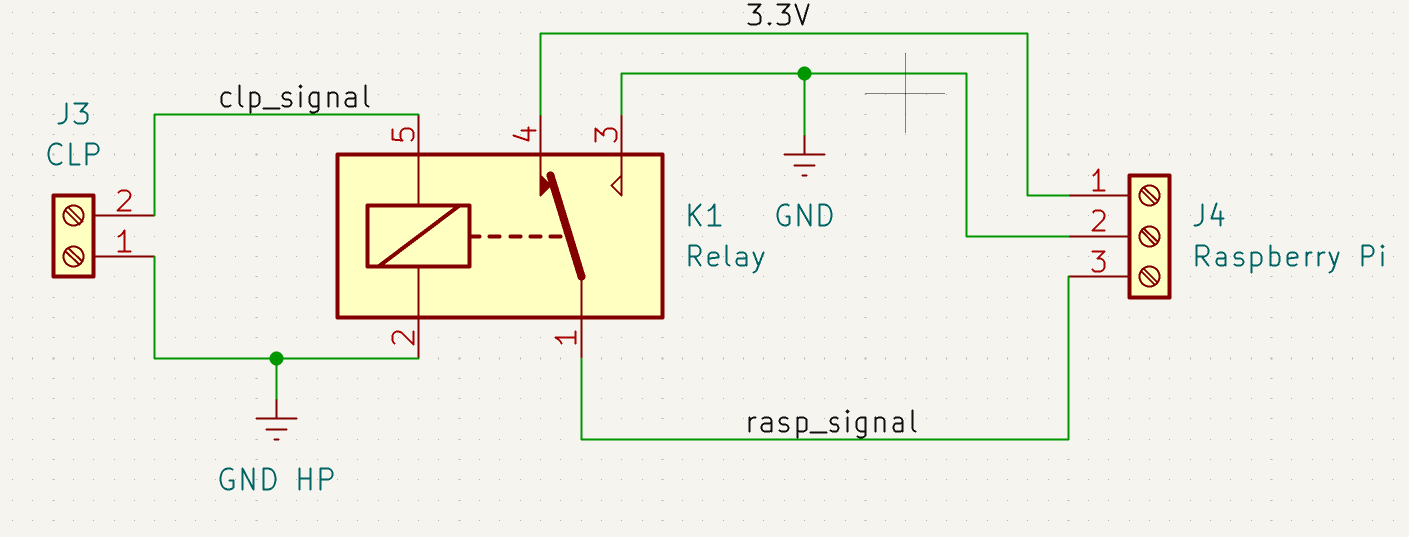
\includegraphics[scale=0.15]{Figuras/esquematico_clp_rasp.png}
    \caption{Esquemático da placa que faz a conexão do sistema industrial com as $GPIOs$ da $Raspberry$}
    \label{fig:2}
\end{figure}

Por fim, foram desenvolvidas duas placas, evidenciando a simplicidade e eficácia do processo de conversão de tensões, o que reforça a viabilidade da integração entre sistemas legados e modernos. \par

A Figura \ref{fig:clp_rasp_board} referencia a placa que faz a conexão via relé, entre CLP e $Raspberry\ Pi$ e a Figura \ref{fig:rasp_clp_board} a placa que faz a conexão entre a $Raspberry\ Pi$ e o CLP, utilizando o optoacoplador. \par

\begin{figure}[!htb]
    \centering
    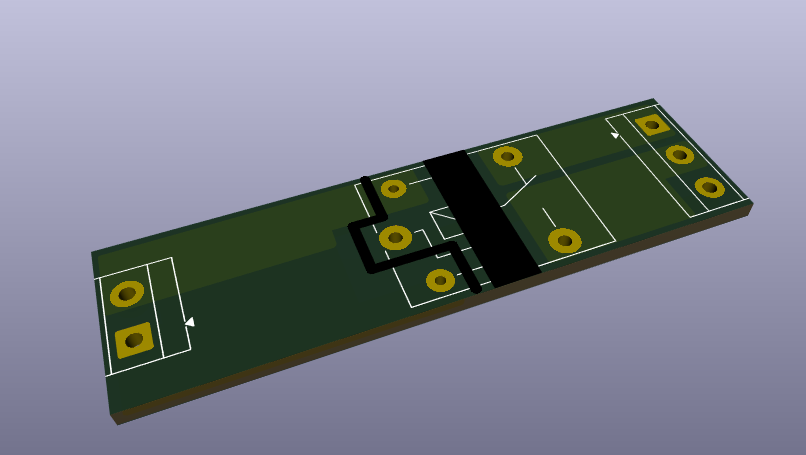
\includegraphics[scale=0.15]{Figuras/placa_clp_rele.png}
    \caption{Modelo 3D da placa que faz a conexão do CLP com a Raspberry Pi}
    \label{fig:clp_rasp_board}
\end{figure}

\begin{figure}[!htb]
    \centering
    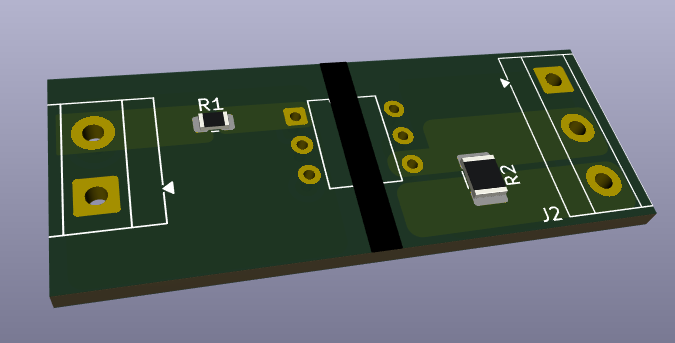
\includegraphics[scale=0.15]{Figuras/placa_rasp_clp.png}
    \caption{Modelo 3D da placa que faz a conexão da Raspberry Pi com o CLP}
    \label{fig:rasp_clp_board}
\end{figure}

Pode-se observar que foram adicionados desenhos específicos à placa (representados pelas linhas pretas), cuja função é atuar como elementos de blindagem eletromagnética, reduzindo a interferência entre os circuitos. Complementarmente, os planos de terra foram distribuídos em camadas distintas da placa, o que contribui para a mitigação de ruídos e reforçam a imunidade eletromagnética do sistema.\par

\subsection{Interface $backend$}
A interface de código $backend$ desenvolvida para a atuação foi baseada no paradigma de programação orientado a objetos \cite{oop}, proporcionando um código mais organizado, legível e com maior manutenibilidade. Essa abordagem facilita adaptações para diferentes cenários, economizando tempo e esforço em futuras implementações. A linguagem utilizada foi $Python$, essa escolha se deu devido a sua simplicidade e eficiência.\par

Inicialmente, foi implementado o código para acesso de baixo nível à $Raspberry\ Pi$, com o objetivo de simplificar o uso e a configuração dos pinos do equipamento. A classe desenvolvida adota uma arquitetura baseada em interfaces, que consiste na definição de um contrato de métodos que devem ser obrigatoriamente implementados pelas classes que a utilizam. Essa abordagem promove a padronização, facilita a extensibilidade do código e assegura a independência entre módulos, aumentando a modularidade e a facilidade de manutenção e atualização do sistema.\par

Desse modo, optou-se pelo uso de interfaces para permitir a modularização entre diferentes tipos de placas controladoras, de modo que, mantendo-se a assinatura dos métodos definidos na interface, novas implementações possam ser integradas ao sistema sem a necessidade de alterações no código principal, assegurando flexibilidade e escalabilidade, fundamentais em cenários que podem ser alterados.\par

Para a construção do objeto, é necessário passar uma lista que, caso utilizada, especifica os pinos a serem configurados como entradas. Esses pinos são automaticamente inicializados pela classe, otimizando o processo de configuração e facilitando eventuais procedimentos de depuração durante o desenvolvimento e a validação do sistema, permitindo assim o acesso simplificado aos comandos de controle dos $GPIOs$ da placa.\par

A Figura \ref{fig:3} representa o diagrama $Unified\ Modeling\ Language\ (UML)$ \cite{uml} das classes de $GPIO$.\par

\begin{figure}[!htb]
    \centering
    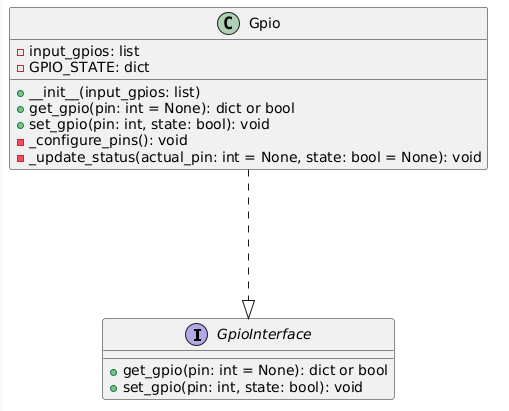
\includegraphics[scale=0.35]{Figuras/diagrama_uml_gpio.png}
    \caption{Diagrama $UML$ da orientação a objeto utilizada para as $GPIOs$}
    \label{fig:3}
\end{figure}

Adicionalmente, desenvolveu-se uma classe específica para definir o objeto $Mqtt$, que desempenha um papel fundamental na comunicação de todo o projeto. A classe foi adaptada para seguir a mesma arquitetura baseada em interfaces, permitindo sua substituição ou extensão com outras formas de comunicação, como SSH ou TCP/IP, sem impactar o restante do sistema, visando garantir maior modularidade e flexibilidade. A fim de compatibilizar a nova estrutura, foi implementado um adaptador específico, o qual integra o $Mqtt$ à interface de comunicação de forma padronizada, aumentando assim a robustez e a adaptabilidade do projeto, tornando-o preparado para possíveis evoluções. \par

No construtor dessa classe, foram definidas três variáveis principais: o domínio para conexão, denominado $THINGSBOARD\_HOST$, o $token$ de acesso, chamado $ACCESS\_TOKEN$, e um dicionário apelidado de $requests$. O $token$ de acesso adiciona uma camada essencial de segurança, protegendo o sistema contra acessos não autorizados durante a troca de dados entre o circuito legado e a interface desenvolvida.\par

Por sua vez, o dicionário $requests$ desempenha um papel fundamental na camada de abstração superior. Ele permite que o sistema especifique as variáveis requisitadas e o método de atuação correspondente à requisição. Quando uma solicitação é recebida, a classe utiliza esse dicionário para realizar o direcionamento da requisição e a enviando ao método apropriado para a manipulação do dado. Essa abordagem modular e organizada torna o sistema mais versátil e escalável, facilitando a integração e o tratamento eficiente das comunicações entre as diferentes camadas do projeto. \par

O diagrama UML, representado pela Figura \ref{fig:diagrama_uml_conexão} exemplifica como foi desenvolvida a arquitetura da comunicação.
\begin{figure}[!htb]
    \centering
    \includegraphics[scale=0.3]{Figuras/diagrama_uml_conexão.png}
    \caption{Diagrama $UML$ da orientação a objeto utilizada para a comunicação}
    \label{fig:diagrama_uml_conexão}
\end{figure}

Com o objetivo de integrar o controle de sinais digitais aos mecanismos de comunicação externos, foi desenvolvida a classe $GpioCommunicationBridge$. Esta classe atua como uma ponte entre a interface de comunicação e a interface de controle de $GPIOs$, proporcionando uma abstração de alto nível que permite monitorar e enviar dados de eventos de pinos de forma desacoplada.\par

A arquitetura foi construída com base no uso de interfaces, assegurando que tanto o sistema de comunicação quanto o de controle de $GPIO$ possam ser substituídos ou adaptados sem impacto na lógica principal da aplicação, desde que respeitem as assinaturas estabelecidas. A classe $GpioCommunicationBridge$ recebe, em sua construção, instâncias que implementam as interfaces de comunicação e de $GPIO$, respectivamente, o que permite a fácil integração de diferentes protocolos e plataformas de $hardware$.\par

Durante a execução, a classe realiza a detecção de alterações no estado dos pinos configurados e publica os eventos detectados através da camada de comunicação disponível. Dessa forma, ela proporciona uma separação clara de responsabilidades entre captura de eventos físicos e transmissão de dados.\par

A Figura \ref{fig:diagrama_uml_gpio_communication} representa um diagram $UML$ de como os códigos se integram.\par
\begin{figure}[!htb]
    \centering
    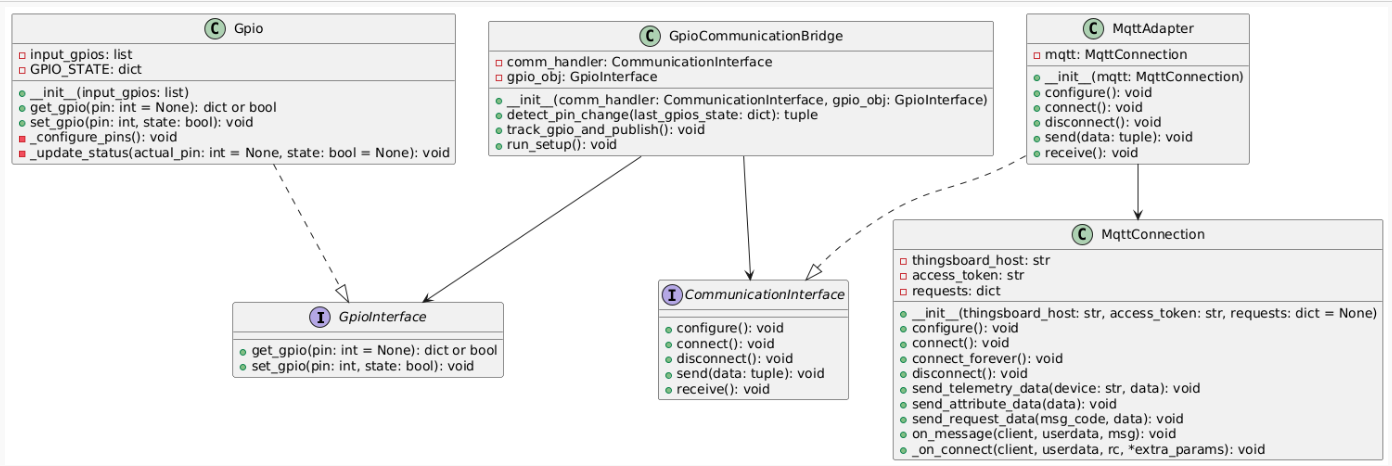
\includegraphics[scale=0.17]{Figuras/diagrama_uml_gpio_communication.png}
    \caption{Diagrama $UML$ da orientação a objeto utilizada para a integração das classes}
    \label{fig:diagrama_uml_gpio_communication}
\end{figure}

\subsection{Interface $frontend$}

A interface $frontend$ do projeto utiliza as ferramentas integradas já oferecidas pela plataforma $ThingsBoard$, aproveitando sua capacidade de abstrair elementos como animações de $widgets$ e a interação entre o usuário e a $Raspberry\ Pi$. O primeiro passo no desenvolvimento da interface foi analisar as funcionalidades necessárias para cobrir toda a operação do sistema. \par

Nesse contexto, considerou-se a utilização de dois elementos principais: uma chave e um $LED$ virtual. O primeiro funciona como uma botoeira industrial, permitindo ao operador iniciar o processo industrial. Sua comunicação é realizada por dois métodos de requisição. Enquanto um método verifica a posição do pino para determinar se a chave deve ser exibida como ligada ou desligada, ou seja, esse controle facilita o acompanhamento e a interação do operador com o sistema em tempo real. Já o outro método tem como responsabilidade informar à placa qual o pino alterado e para qual nível lógico ele deve ser alterado.\par

O segundo elemento, o $LED$ virtual, tem como objetivo indicar ao operador se o sensor está sendo acionado no sistema industrial. Com isso, a representação gráfica proporciona um $feedback$ visual tornando o sistema mais intuitivo. \par 

A Figura \ref{fig:5} representa o diagrama de funcionamento  da interface $frontend$ do sistema. \par  

\begin{figure}[!htb]
    \centering
    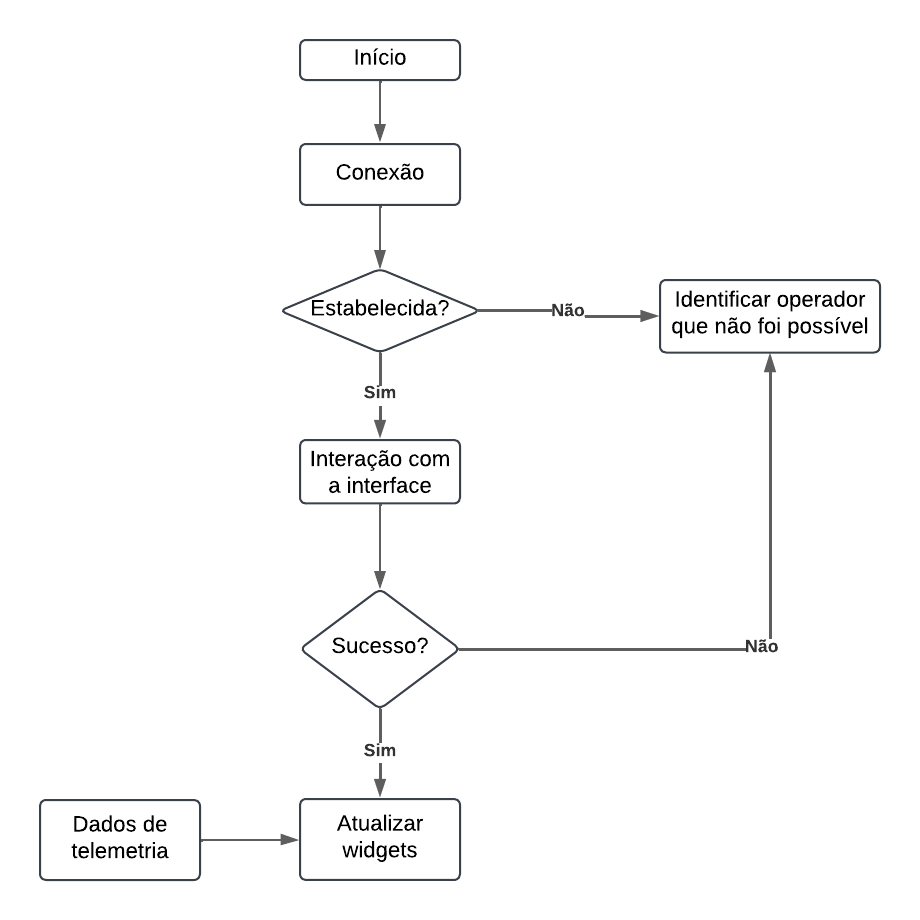
\includegraphics[scale=0.17]{Figuras/fluxograma_frontend.png}
    \caption{Fluxograma da interface $frontend$}
    \label{fig:5}
\end{figure}

\subsection{Integração $frontend/backend$}
\label{SeçãoIV4}
Para descrever o desenvolvimento da integração das interfaces do sistema, é necessário compreender como a comunicação do projeto é estruturada. O $ThingsBoard$ utiliza um conceito central chamado tópicos, que possibilitam a troca de informações e comandos entre o dispositivo e a plataforma. Esses tópicos desempenham papéis específicos na comunicação e são categorizados da seguinte forma: \par 

\begin{itemize}
\item Tópico de telemetria: Responsável pelo envio contínuo de dados provenientes de sensores conectados ao dispositivo. Ele permite monitorar em tempo real as condições do sistema, transferindo informações como temperatura, corrente ou status do equipamento.
\item Tópico de requisição: Utilizado para realizar os $Remote\ Procedure\ Calls\ (RPC)$. Nesse processo, a plataforma envia um comando ao dispositivo com o objetivo de realizar uma ação específica. O dispositivo, por sua vez, executa o comando e aguarda para responder.
\item Tópico de resposta ($response$): Um complemento do tópico de requisição, que lida com as respostas às chamadas $RPC$ realizadas. Ele assegura a comunicação bidirecional, permitindo a plataforma confirmar se o dispositivo executou a ação requisitada corretamente.
\item Tópico de atributos: Responsável por atualizar a interface gráfica com informações relevantes sobre o sistema. Ele permite personalizar e dinamizar a interface, refletindo as mudanças nos estados do sistema em tempo real para o usuário.
\end{itemize}

Esses tópicos trabalham de forma integrada possibilitando uma comunicação robusta e confiável entre o dispositivo e a plataforma. Portanto, isso garante a sincronização das ações e informações do sistema. \par

No contexto do projeto desenvolvido, os dados coletados pelo sensor são enviados para a plataforma $ThingsBoard$ utilizando o tópico de telemetria de forma síncrona, ou seja, com um fluxo contínuo e regular. Por outro lado, os tópicos restantes (como requisições e respostas) operam de maneira assíncrona, sendo disparados conforme necessário, geralmente por ações realizadas pelo operador, como iniciar ou finalizar um processo industrial. \par

Entretanto, essa arquitetura apresenta uma vulnerabilidade: o envio descontrolado de dados para a rede pode causar um transbordamento de informações, sobrecarregando a conexão. Esse problema pode levar à instabilidade na comunicação e, eventualmente, à perda de dados, comprometendo o desempenho do sistema. \par

Para superar essa limitação e garantir maior robustez, foi implementada uma lógica que otimiza a comunicação. Essa lógica estabelece que os dados só são enviados para a plataforma quando ocorre uma mudança significativa nos valores monitorados e enviando somente aquilo que sofreu alteração. Esse mecanismo evita o envio redundante de informações, reduzindo o tráfego na rede e, consequentemente, assegurando uma conexão mais estável e confiável. Essa abordagem não apenas protege o sistema contra possíveis falhas, mas também melhora sua eficiência ao minimizar o consumo de recursos da rede. \par

A Figura \ref{fig:6} apresenta um fluxograma que ilustra de maneira clara e objetiva os principais pontos abordados neste tópico, proporcionando uma visão mais ilustrativa do funcionamento do sistema e das etapas discutidas. \par

\begin{figure}[!htb]
    \centering
    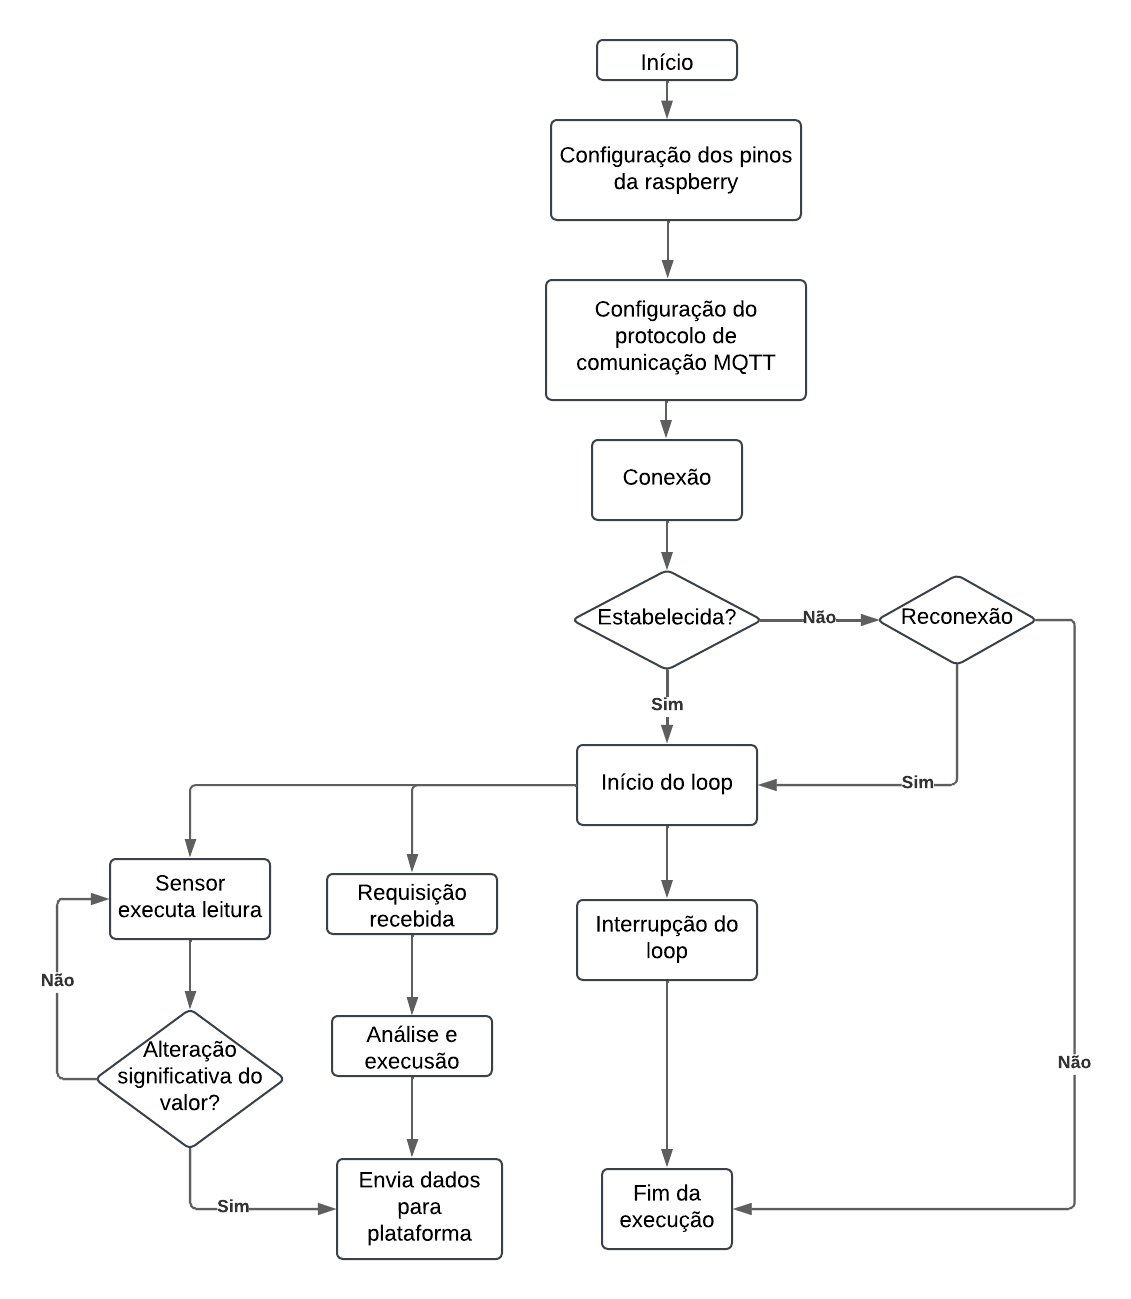
\includegraphics[scale=0.16]{Figuras/fluxograma_front_backend.png}
    \caption{Fluxograma da interface $frontend$ e $backend$}
    \label{fig:6}
\end{figure}


\section{Configuração do $ThingsBoard$}

Essa seção funcionará como um guia para a criação de um $dashboard$ na plataforma $ThingsBoard$, adicionando elementos de monitoramento e de acionamento que serão integrados ao $framework$.\par

\subsection{Monitoramento}
O sistema de monitoramento se refere aos dados enviados de forma contínua, conforme já mencionado na seção \ref{SeçãoIV4}. Esses dados estão associados a variáveis específicas, cujo valor é transmitido pela rede para visualização pelo operador, garantindo o monitoramento em tempo real. \par

Na interface gráfica do $ThingsBoard$, o primeiro passo é adicionar um $widget$ que mostre visualmente o valor desejado. Para esta demonstração, utilizaremos um $LED$ virtual, que pode ser encontrado no caminho $Widgets\ >\ Control\ Widgets\ >\ Led\ Indicator$. \par

Após adicionar o $widget$, é necessário o vincular ao dispositivo transmissor dos dados. Neste caso, a $RaspberryPi4$ é responsável pelo envio das informações de telemetria. A Figura \ref{fig:7} demonstra essa operação. \par

\begin{figure}[!htb]
    \centering
    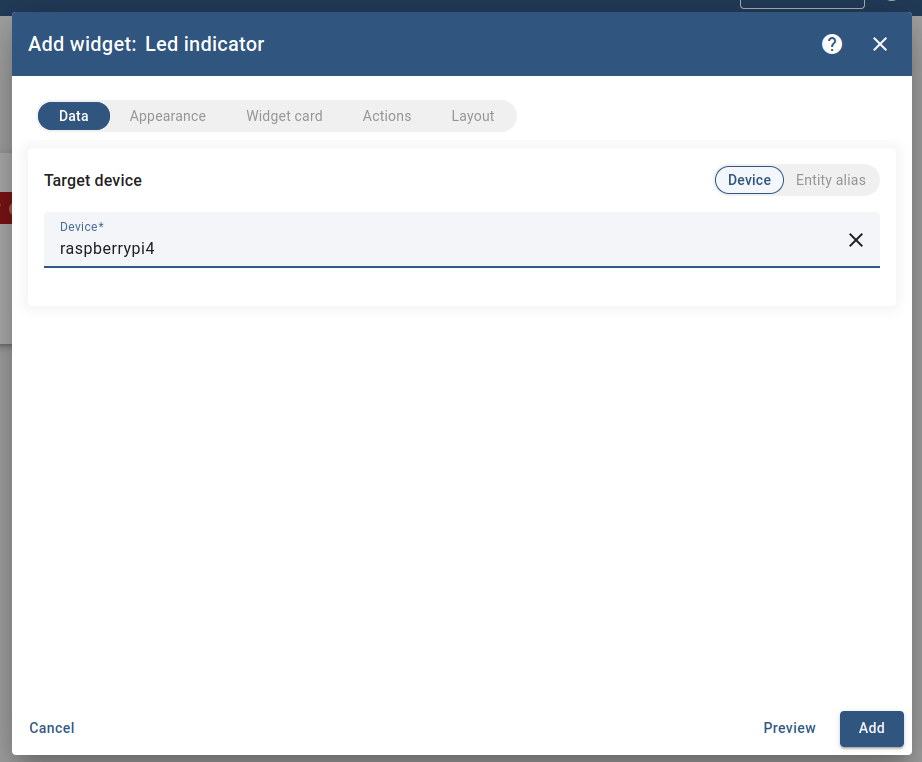
\includegraphics[scale=0.2]{Figuras/selecionando_device_thingsboard.png}
    \caption{Configurando o $device$ de telemetria}
    \label{fig:7}
\end{figure}

Com o dispositivo de telemetria já selecionado, procede-se à configuração do modo de recebimento dos dados. Para este caso, foi escolhida a opção capaz de verificar o status de telemetria em intervalos de tempo, permitindo a atualização contínua da interface gráfica. Essa configuração pode ser encontrada na aba de "Aparência do $widget$". \par

Em seguida, define-se o nome da variável que armazenará o valor de telemetria. Para a integração com o $framework$ desenvolvido, este deve ser relacionado ao número do pino configurado como entrada. Esse também será utilizado para vincular os dados recebidos ao $widget$ configurado. Por fim, a operação completa pode ser visualizada na Figura \ref{fig:8}.

\begin{figure}[!htb]
    \centering
    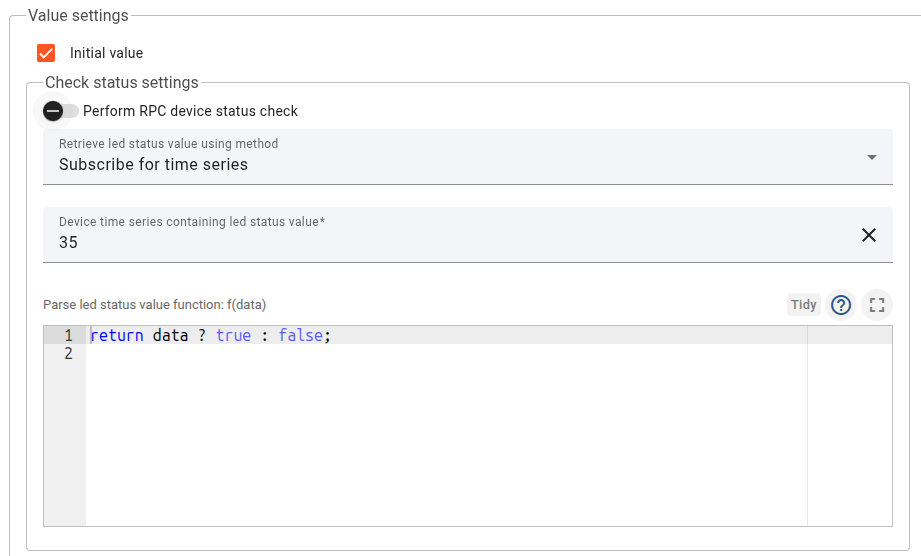
\includegraphics[scale=0.2]{Figuras/config_variavel.png}
    \caption{Configurando a variável de telemetria}
    \label{fig:8}
\end{figure}

Com essas configurações concluídas, é possível visualizar as alterações no valor do $LED$ diretamente no sistema, refletindo as mudanças enviadas pelo dispositivo em tempo real. A Figura \ref{fig:9} ilustra os dois estados do $LED$.

\begin{figure}[!htb]
    \centering
    \begin{minipage}[!]{0.25\linewidth}
        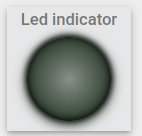
\includegraphics[scale=0.50]{Figuras/led_apagado.png}
    \end{minipage}
    \begin{minipage}[!]{0.25\linewidth}
        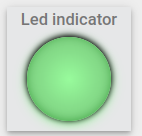
\includegraphics[scale=0.50]{Figuras/led_ativo.png}
    \end{minipage}
    \caption{Exemplo do funcionamento do visualizador de $LED$}
    \label{fig:9}
\end{figure}

\subsection{Acionamento}

Conforme mencionado na Seção \ref{SeçãoIII1}, para controlar o sistema foi utilizada uma chave virtual, responsável por ativar e desativar o sistema. O primeiro passo é adicionar essa chave à área de trabalho. No projeto, a chave utilizada pode ser encontrada no caminho $Widgets\ >\ Control\ Widgets\ >\ Basic\ GPIO\ Control$. \par

Após adicionar o elemento, é necessário vinculá-lo ao dispositivo que está enviando e recebendo os dados, que neste caso é a $Raspberry\ Pi$. \par

Por ser um $widget$ projetado para aplicações com $Raspberry\ Pi$, ele oferece alta compatibilidade com o sistema, reduzindo a necessidade de configurações adicionais. Além disso, é possível personalizar os nomes dos métodos de requisição, o que pode ser útil em aplicações mais específicas. Para ajustar essa configuração, basta acessar a aba "Aparência do $widget$" e localizar os campos correspondentes às requisições $get$ e $set$ do dispositivo. A Figura \ref{fig:10} ilustra essa configuração. \par

\begin{figure}[!htb]
    \centering
    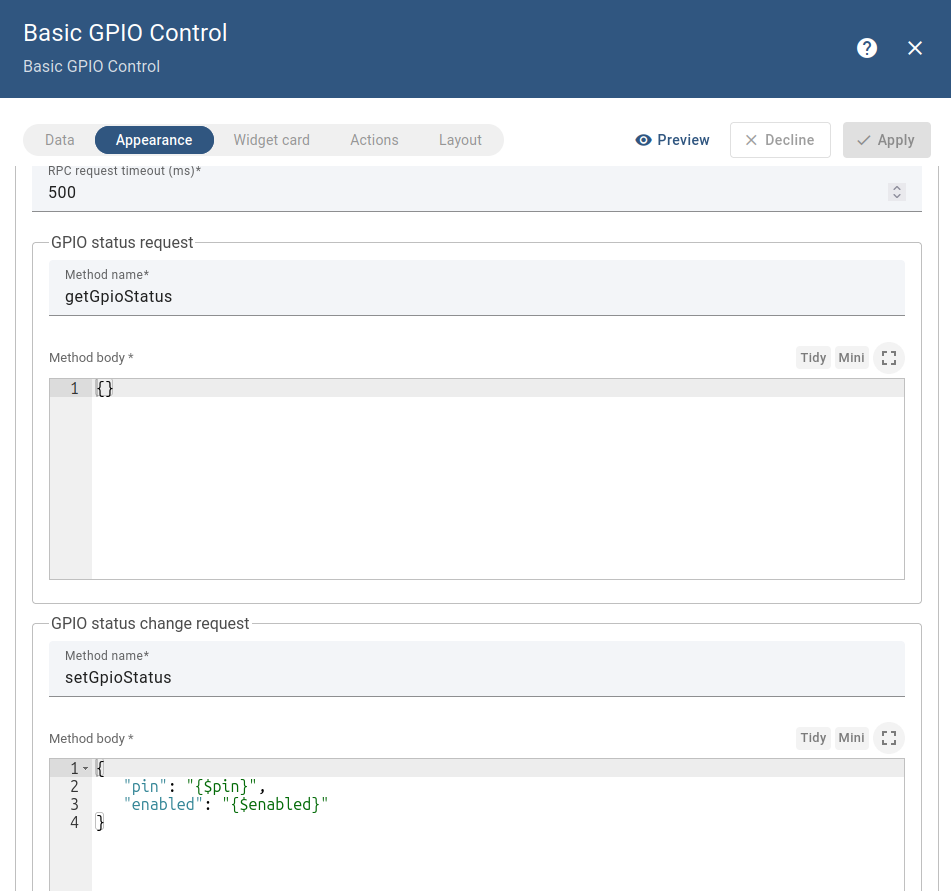
\includegraphics[scale=0.20]{Figuras/metodos_chave.png}
    \caption{Configuração dos métodos da chave}
    \label{fig:10}
\end{figure}

Com essas configurações realizadas, é possível controlar remotamente as $GPIOs$ da $Raspberry\ Pi$ e, consequentemente, operar o sistema legado. As Figuras \ref{fig:11} e \ref{fig:12} ilustram o funcionamento desse $widget$. \par

\begin{figure}[!htb]
    \centering
    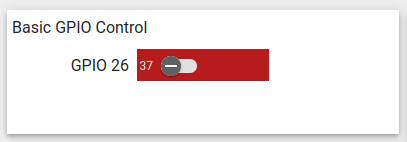
\includegraphics[scale=0.55]{Figuras/chave_desligada.png}
    \caption{Demonstração da $GPIO$ de controle desligada}
    \label{fig:11}
\end{figure}

\begin{figure}[!htb]
    \centering
    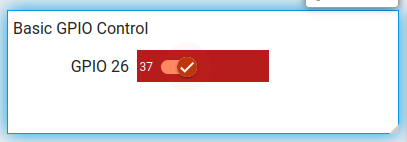
\includegraphics[scale=0.55]{Figuras/chave_ligada.png}
    \caption{Demonstração da $GPIO$ de controle ligada}
    \label{fig:12}
\end{figure}

\section{Configuração do $framework$}
Essa seção funcionará como um guia para a utilização e integração do $framework$ desenvolvido, destacando sua praticidade e acessibilidade. De modo a facilitar futuras modificações e personalizações, a arquitetura do sistema foi projetada para separar trechos específicos do código onde o usuário pode intervir, realizando adaptações de acordo com as necessidades da aplicação.\par

O $framework$ foi inspirado em ferramentas populares de desenvolvimento embarcado, como o $Arduino IDE$ \cite{arduino_ide} ou o $STM32CubeIDE$ \cite{stm}, que delimitam regiões do código destinadas à inserção de comandos personalizados, o sistema implementado apresenta áreas claramente marcadas para alterações seguras.\par

\subsection{Placa de controle}
Primeiramente, dada a configuração da $Raspberry\ Pi$, é necessário adicionar os pinos que serão utilizados como entrada pelo sistema. Esses valores devem ser fornecidos por meio de uma lista de números inteiros, os quais mapeiam os pinos de entrada. Para alterar essa configuração, basta modificar o valor da variável “$INPUT\_PINS$” para os pinos desejados. \par

Ao fornecer esses à classe, ela automaticamente realiza a configuração necessária para o correto funcionamento do programa. A Figura \ref{fig:framework_rasp} demonstra essa configuração. \par

\begin{figure}[!htb]
    \centering
    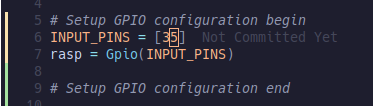
\includegraphics[scale=0.55]{Figuras/gpio_framework.png}
    \caption{Trecho de código da configuração dos $GPIOs$}
    \label{fig:framework_rasp}
\end{figure}

\subsection{Conexão com $ThingsBoard$}
Para configurar o servidor, basta alterar as variáveis “$THINGSBOARD\_HOST$” e “$ACCESS\_TOKEN$”. A plataforma utilizada para a validação deste projeto foi a "$demo.thingsboard.io$”, contudo essa configuração não se limita a essa plataforma. Neste caso, o $token$ de acesso é obtido a partir do dispositivo configurado na plataforma $ThingsBoard$. \par

Com o objetivo de melhorar a legibilidade do código, o tratamento dos requerimentos fica sob responsabilidade do operador, que deve configurar adequadamente. Para isso, é necessário ajustar o dicionário "$requests$". Por sua vez, este dicionário mapeia a variável de requerimento recebida do servidor para o método que será utilizado. O trecho de código que ilustra essa configuração pode ser visto na Figura \ref{fig:13}.

\begin{figure}[!htb]
    \centering
    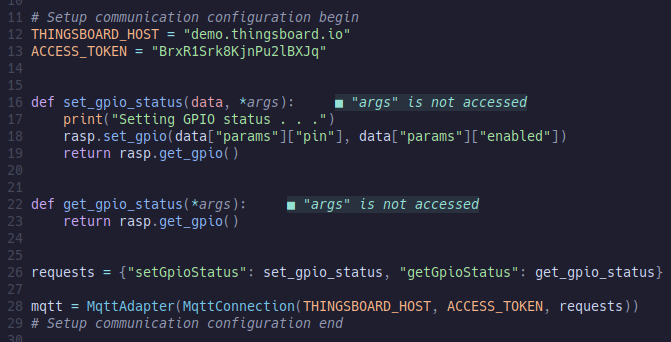
\includegraphics[scale=0.30]{Figuras/comunicação_framework.png}
    \caption{Trecho de código da configuração da comunicação}
    \label{fig:13}
\end{figure}

No trecho de código, demonstrado pela Figura \ref{fig:13}, cria-se os métodos "$set\_gpio\_status$" e "$get\_gpio\_status$", que são essenciais para o funcionamento do sistema legado idealizado. Esses métodos são associados a uma chave do dicionário "$requests$". É importante ressaltar que a chave do dicionário deve ter o mesmo nome da variável configurada dentro do $widget$. Caso contrário, os dados serão perdidos durante a comunicação, comprometendo o funcionamento correto do sistema. \par

\subsection{Aplicação}
 Na simulação proposta (o monitoramento de embalagens em uma linha de produção), essas regiões foram previamente preenchidas com exemplos de uso funcional, servindo tanto para validação do sistema quanto para guiar o desenvolvimento de aplicações futuras. Essa abordagem modular proporciona maior agilidade no ajuste do sistema para novas tarefas, reduzindo o esforço de reescrita e mantendo a estrutura principal de monitoramento e comunicação consistente e robusta. A Figura \ref{fig:14} mostra o trecho de código em questão. \par

\begin{figure}[!htb]
    \centering
    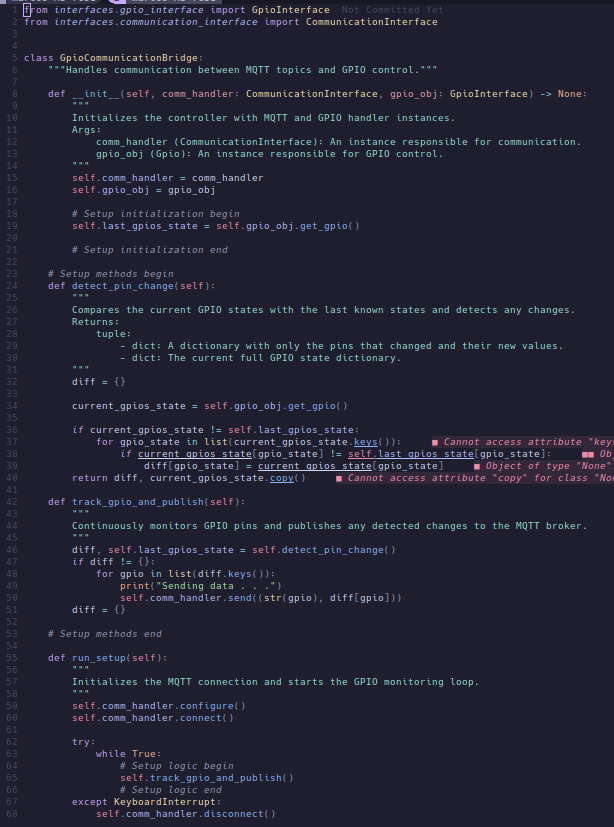
\includegraphics[scale=0.273]{Figuras/communication_gpio_controller_preenchido.png}
    \caption{Trecho de código com delimitação de áreas destinadas à personalização do usuário.}
    \label{fig:14}
\end{figure}

\section{Conclusão}
O desenvolvimento deste projeto demonstrou a viabilidade da integração entre sistemas legados e tecnologias modernas de comunicação baseadas em $IoT$, utilizando arquiteturas modulares, escaláveis e de fácil manutenção. A implementação de interfaces para abstração do controle de $GPIOs$ e das camadas de comunicação, aliadas à aplicação de padrões de projeto como $Adapter$, permitiu criar um sistema altamente adaptável, preparado para suportar diferentes plataformas de hardware e protocolos de comunicação.\par

A utilização de dispositivos como o optoacoplador 4N25 e o relé para isolamento elétrico garantiu a segurança e a integridade dos componentes modernos frente aos sistemas industriais, preservando a confiabilidade do ambiente de operação. A integração com a plataforma $ThingsBoard$ permitiu validar a comunicação remota de forma intuitiva e eficiente, evidenciando o potencial de ampliação e aplicabilidade da solução em ambientes industriais e laboratoriais reais.\par

Além disso, a estratégia de otimização no envio de dados, transmitindo apenas alterações relevantes, contribuiu para a eficiência da rede e para a robustez da comunicação, características essenciais em aplicações de monitoramento contínuo.\par

Com a estrutura proposta, o sistema mostrou-se versátil, capaz de se adaptar a diferentes contextos de aplicação sem a necessidade de reescrita significativa de código. A modularidade obtida representa um avanço significativo no desenvolvimento de soluções de modernização de plantas legadas, proporcionando uma alternativa de baixo custo, alta eficiência e grande potencial de expansão.\par

Por fim, o projeto contribui para o fortalecimento do uso de tecnologias de $IoT$ em cenários industriais tradicionais, aproximando-os das novas demandas de automação, controle e monitoramento remoto, alinhando-se às tendências de transformação digital no setor.\par
	
\section{Agradecimentos}
Agradeço primeiramente à minha família, pelo apoio incondicional, incentivo e compreensão ao longo de toda a minha trajetória acadêmica. Sem a base sólida que me proporcionaram, esta conquista não seria possível. \par

Aos meus amigos, que caminharam comigo durante a jornada da faculdade, oferecendo apoio, companheirismo e palavras de incentivo nos momentos de dificuldade e celebração nas vitórias. \par

Ao professor Dr. Rodrigo Maximiano, meu orientador, pela orientação, apoio e contribuições essenciais para a realização deste trabalho. \par

A todos que, direta ou indiretamente, contribuíram para a realização deste projeto, deixo aqui meu mais sincero agradecimento. \par
	


\bibliographystyle{unsrt}
\bibliography{referencias}
		
\end{document}